% Chapter 6

\chapter{Tests and Evaluation} % Main chapter title

\label{chap:Chapter6} % For referencing the chapter elsewhere, use \ref{chap:Chapter6} 

%----------------------------------------------------------------------------------------

This chapter outlines the testing and evaluation processes crucial to achieving the project’s objectives. It begins with Section 6.1, which focuses on the tests conducted on the merging unit ()publisher of IEC 61850-9-2-SV, ensuring it performs accurately under various conditions. Section 6.2 details the testing of the subscriber, examining its ability to receive and process the data correctly. Finally, Section 6.3 evaluates the algorithm, particularly the state machine implemented to select the best sample of the analog signal. Throughout this chapter, rigorous testing approaches are emphasized, highlighting the steps taken to validate the algorithm's performance and secure the project's overall success. Initially, the testing path wasn’t entirely clear, but as it progressed, the necessary methods and solutions were identified to ensure the algorithm’s successful validation.

\section{Test of Publisher of IEC~61850-9-2-SV}

The testing phase for the publisher was critical to ensure its proper functionality, confirm that the data structures were correctly constructed, and verify that the checksum maintained packet integrity, all in strict compliance with the IEC~61850 standard.

Initial tests focused on validating that the publisher was generating Sampled Value (SV) packets accurately, with values consistent with the configured parameters. It was equally important to verify that the subscriber was correctly receiving and processing these transmitted packets. Wireshark software was extensively employed to capture and analyze the packets, ensuring that all content was transmitted as expected. Throughout development, several issues emerged, but each was methodically resolved to ensure the publisher's reliable performance and seamless communication.

Figure~\ref{fig:simple_sv} Below is a Wireshark capture that illustrates the integrity of the acquired packets and their identification as SV packets.

\begin{figure}[tbh]
	\centering
	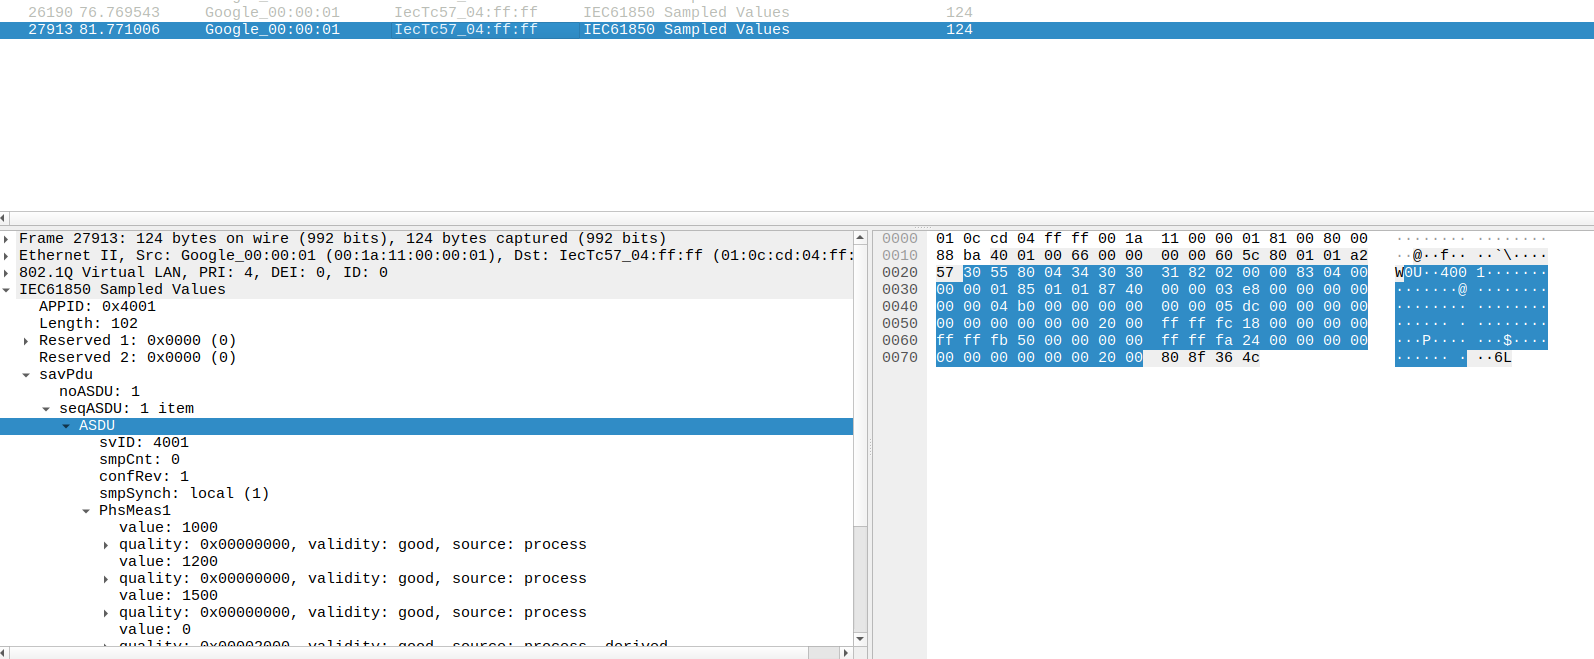
\includegraphics[width=1.00\textwidth, keepaspectratio]{ch6/assets/simple_sv.png} % Reduce to 90% of the text width
	\caption{Wireshark view of the SV packets.}
	\label{fig:simple_sv}
\end{figure}
\FloatBarrier

Figure~\ref{fig:sv_seq_1} The packets are sequentially numbered, ensuring proper identification. The following image demonstrates that the frames are correctly ordered, the field to check it is sample counter as smpcnt.

\begin{figure}[tbh]
	\centering
	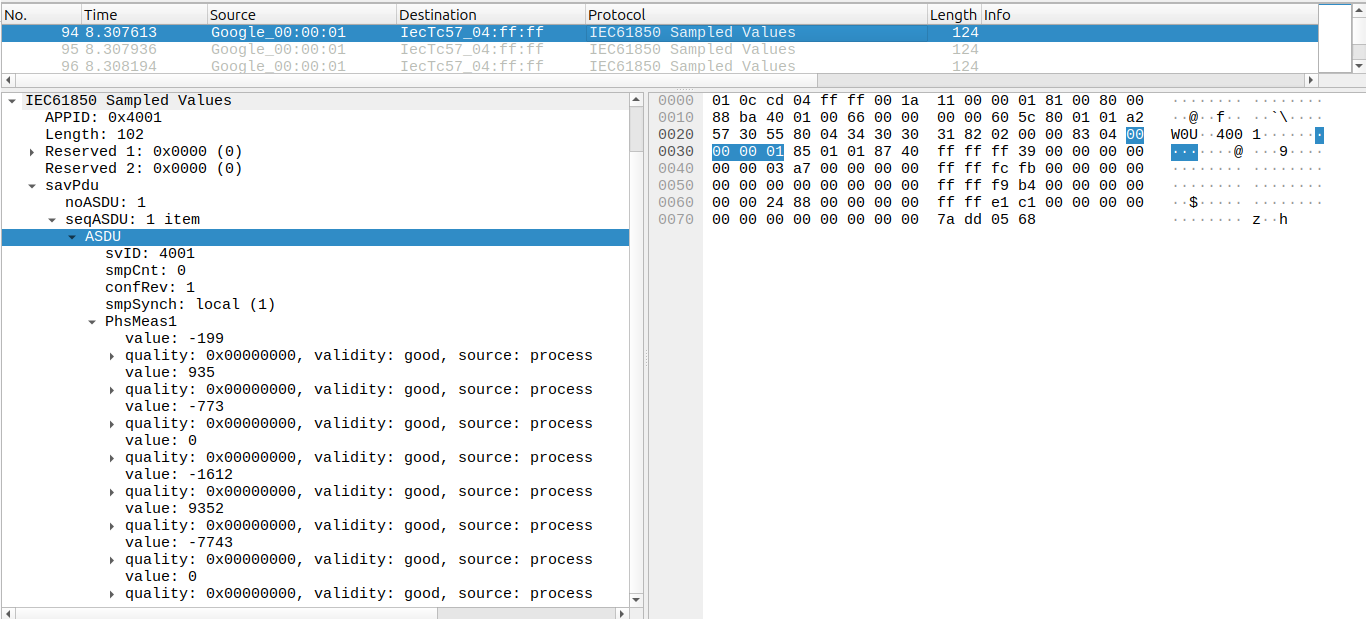
\includegraphics[width=1.00\textwidth, keepaspectratio]{ch6/assets/sv_seq_1.png} % Reduce to 90% of the text width
	\caption{SV packet with sample counter with value 0.}
	\label{fig:sv_seq_1}
\end{figure}
\FloatBarrier

\begin{figure}[tbh]
	\centering
	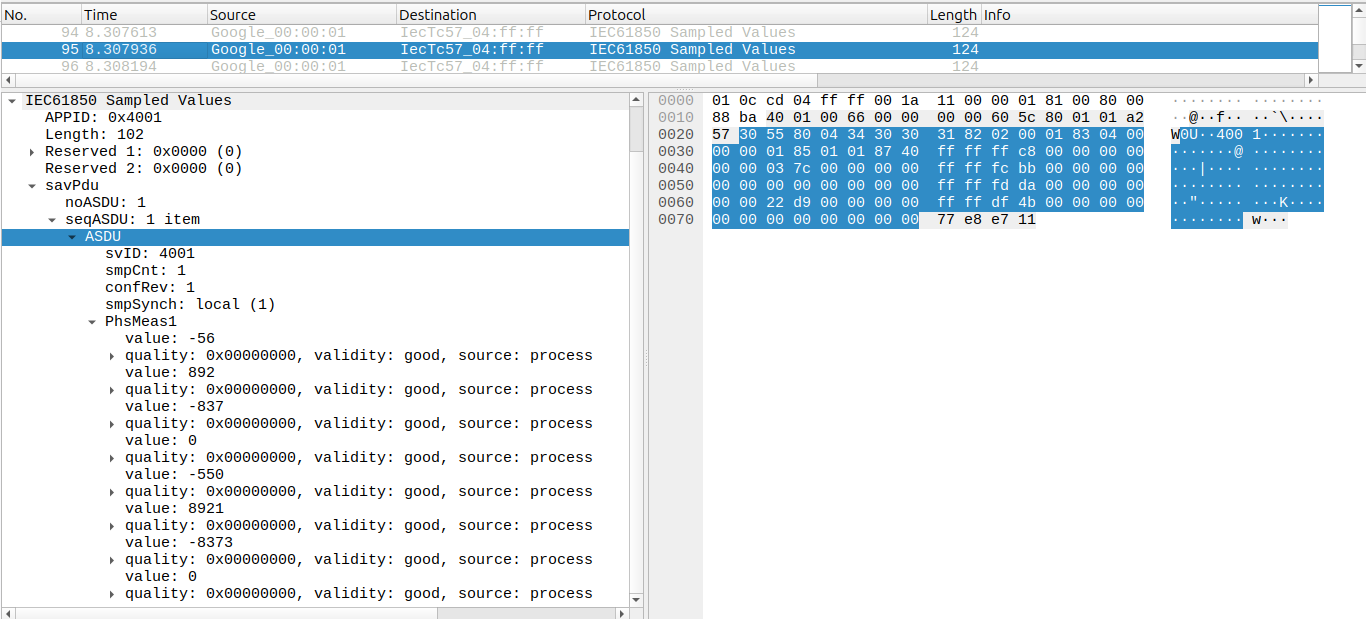
\includegraphics[width=1.00\textwidth, keepaspectratio]{ch6/assets/sv_seq_2.png} % Reduce to 90% of the text width
	\caption{SV packet with sample counter with value 1.}
	\label{fig:sv_seq_2}
\end{figure}
\FloatBarrier

\begin{figure}[tbh]
	\centering
	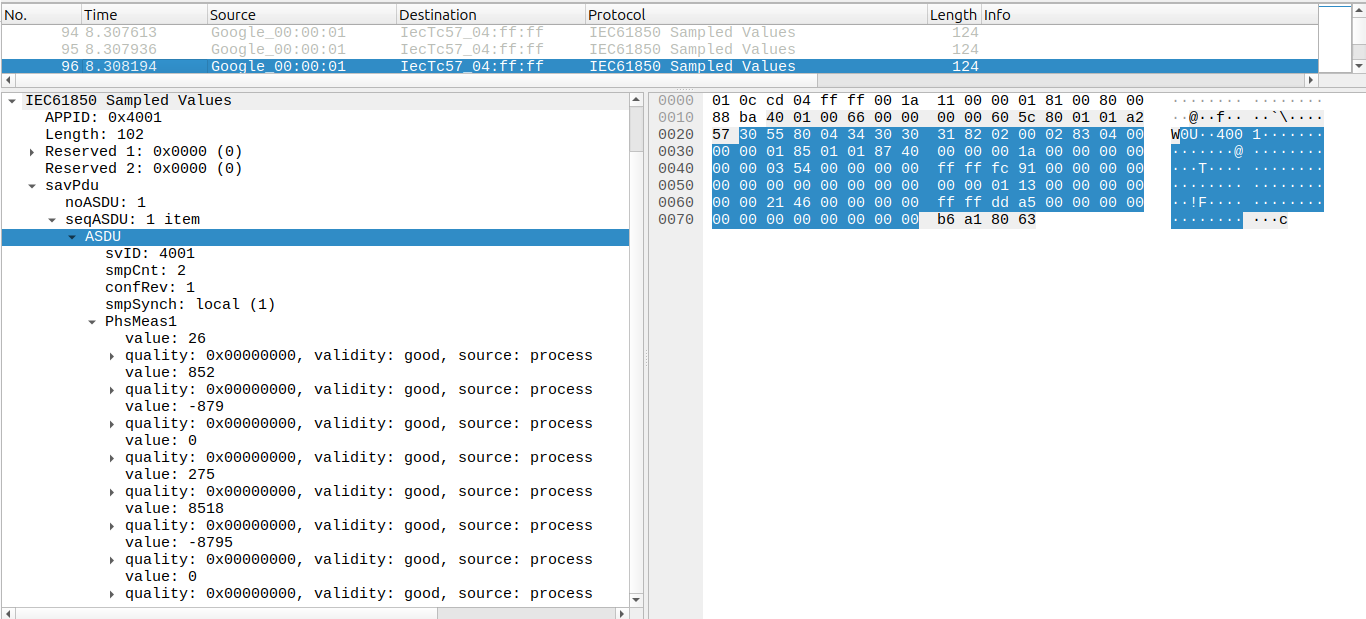
\includegraphics[width=1.00\textwidth, keepaspectratio]{ch6/assets/sv_seq_3.png} % Reduce to 90% of the text width
	\caption{SV packet with sample counter with value 2.}
	\label{fig:sv_seq_3}
\end{figure}
\FloatBarrier

Figure~\ref{fig:sv_seq_bad_1} Here, we showcase samples marked with bad quality, which were used to test the handling of invalid samples and trigger a switch to alternate samples received from another merging unit. The following images provide examples of the transmitted packets.

\begin{figure}[tbh]
	\centering
	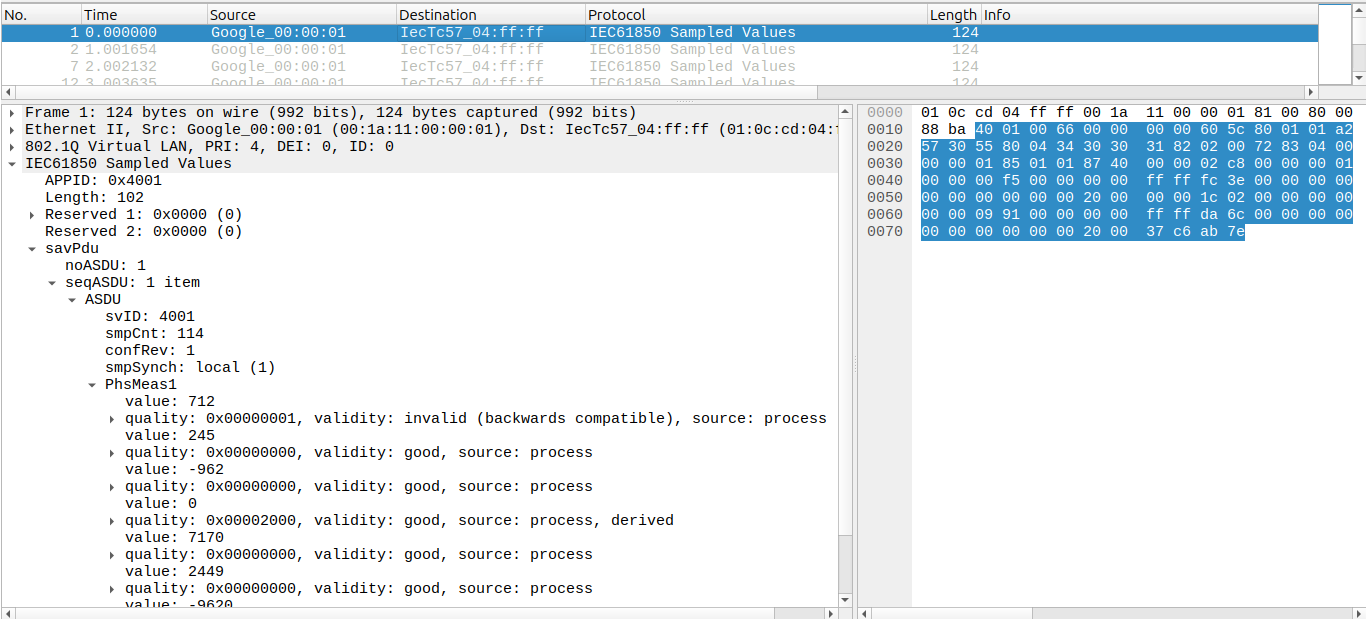
\includegraphics[width=1.00\textwidth, keepaspectratio]{ch6/assets/sv_seq_bad_1.png} % Reduce to 90% of the text width
	\caption{SV packet with bad quality sample counter with value 114.}
	\label{fig:sv_seq_bad_1}
\end{figure}
\FloatBarrier

\begin{figure}[tbh]
	\centering
	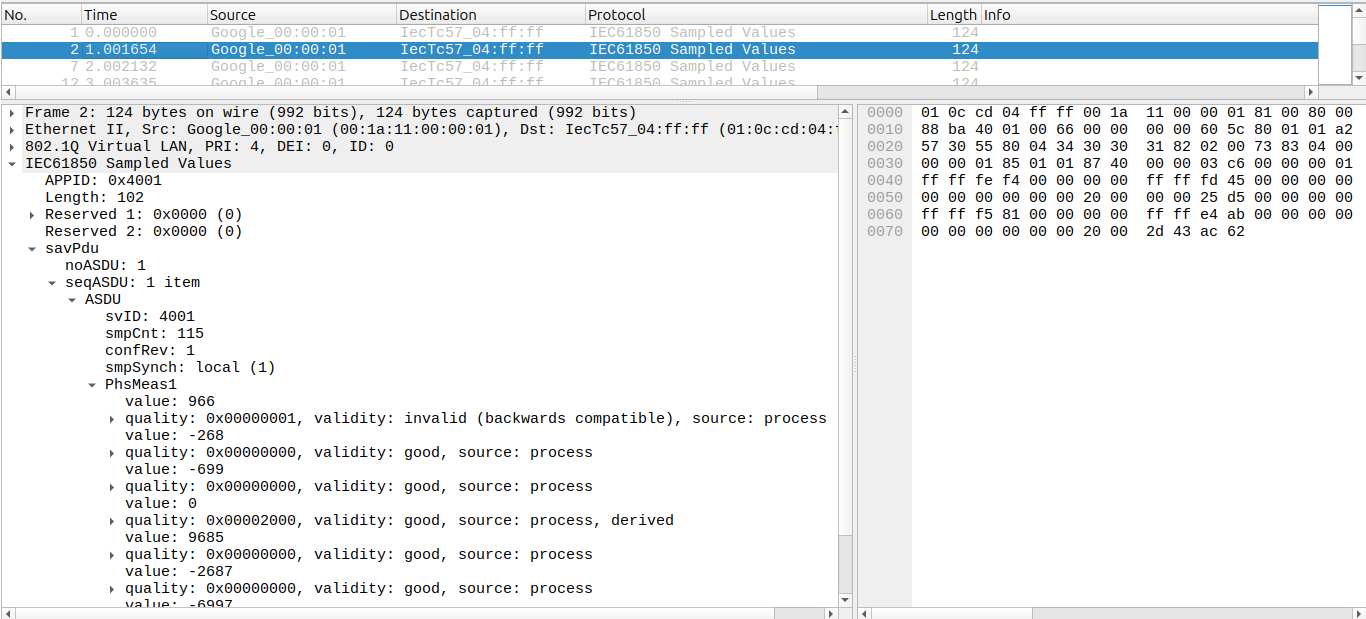
\includegraphics[width=1.00\textwidth, keepaspectratio]{ch6/assets/sv_seq_bad_2.png} % Reduce to 90% of the text width
	\caption{SV packet with bad quality sample counter with value 115.}
	\label{fig:sv_seq_bad_2}
\end{figure}
\FloatBarrier

These comprehensive tests confirm the publisher's correct functionality, ensuring reliable and accurate information exchange between different devices.  The three pictures above show a invalid in the field of quality of the samples, this means I have tested also the way through bad quality samples and ensure the algorithm change which Merging Unit is sending the SV packets, it is also possible to verify the sample counter to realize it is also in order the packets.

\section{Test of Subscriber of IEC~61850-9-2-SV}

The testing phase for the subscriber was essential to ensure it functioned correctly, accurately processed SV packets, and adhered to the IEC~61850 standard.

Initial tests focused on verifying that the subscriber could correctly receive and decode SV packets generated by the publisher. It was crucial to confirm that the subscriber subscribed to the data stream and processed the information as expected. Wireshark was extensively used to monitor and analyze the packet flow, and despite several challenges, each issue was promptly addressed to ensure reliable performance and seamless integration with the publisher.

Throughout testing, both Wireshark and application logs were used to carefully analyze every byte sent and received. This thorough inspection allowed for quick detection of inconsistencies and corrections. Initially, testing on the same machine concealed a problem that became evident only when packets were transmitted across a network: the VLAN information in SV packets was stripped by the operating system when sent to another device. This behavior is normal, as the VLAN data is only necessary for routing but doesn’t reach the application level. Understanding this behavior was crucial for addressing the issue and implementing a solution.

Once the core issues were resolved, testing confirmed the accurate exchange of data, ensuring each byte was correctly serialized and deserialized. This was vital since the state machine relies on precise data to make decisions. Any discrepancies would have caused failures or erratic behavior in the sample selection algorithm. The thorough testing guaranteed that the system operated as intended, free of errors.

Figure~\ref{fig:subscriber_side} Here, we have the wireshark sniffing the information at the subscriber side, and also one packet of the publisher and the subscriber side.

\begin{figure}[tbh]
	\centering
	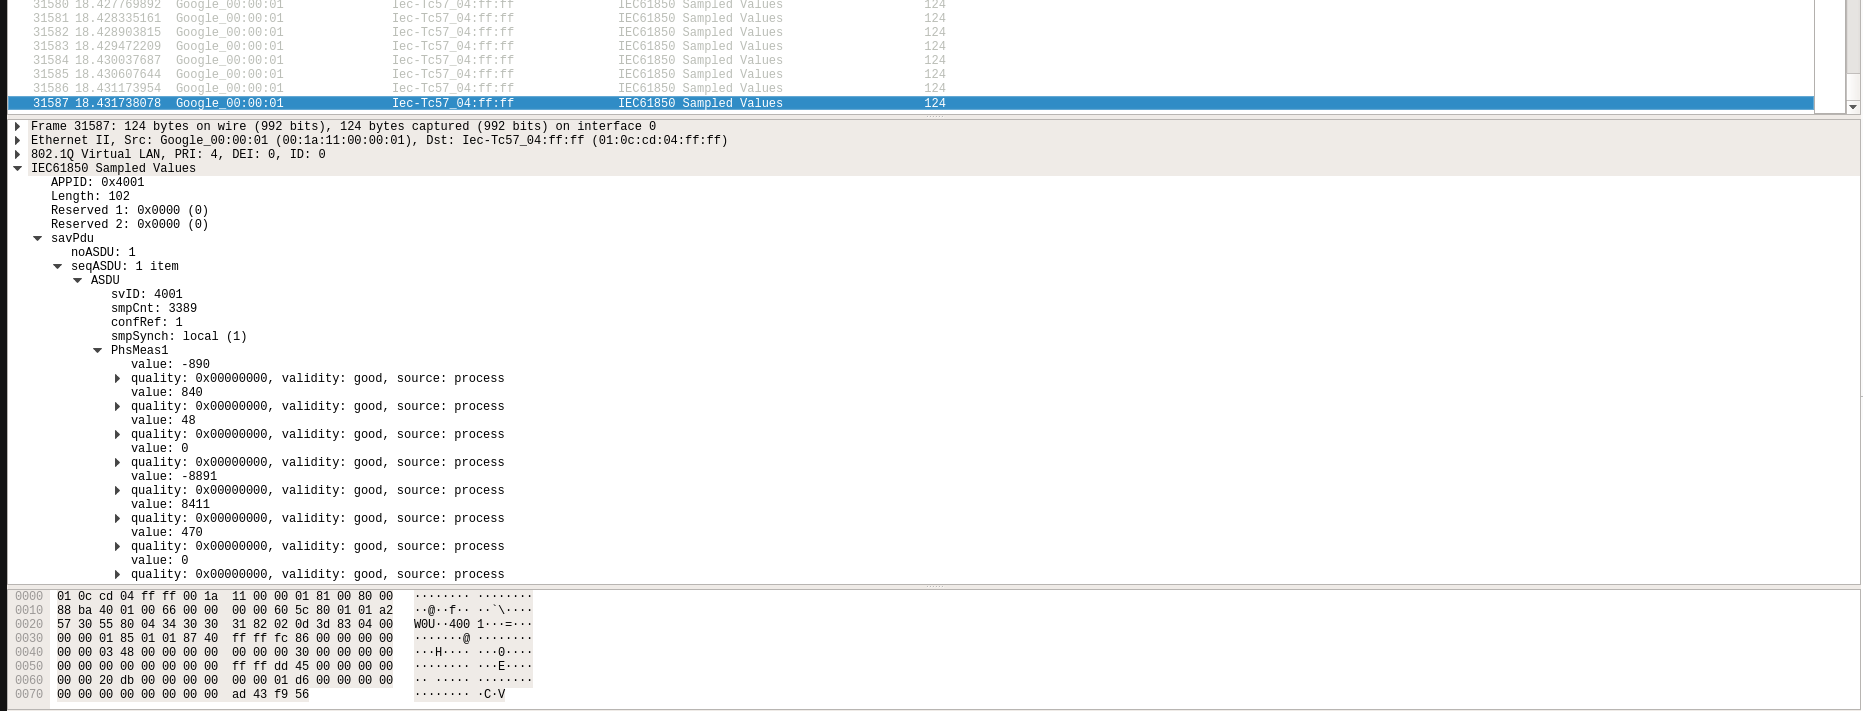
\includegraphics[width=1.00\textwidth, keepaspectratio]{ch6/assets/subscriber_side.png} % Reduce to 90% of the text width
	\caption{SV packet at subscriber side}
	\label{fig:subscriber_side}
\end{figure}
\FloatBarrier

\begin{figure}[tbh]
	\centering
	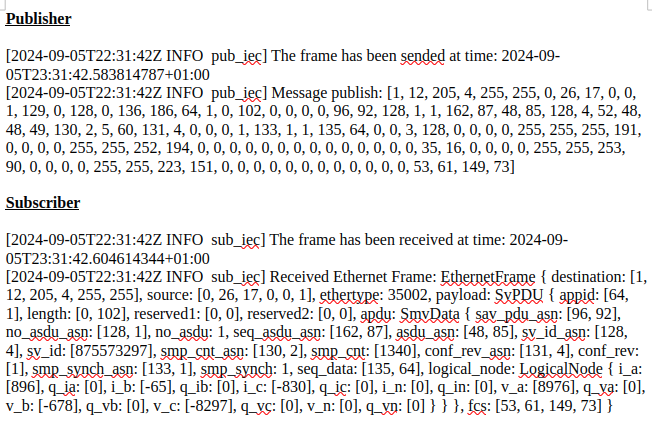
\includegraphics[width=0.85\textwidth, keepaspectratio]{ch6/assets/information_packet_sub_pub.png} % Reduce to 90% of the text width
	\caption{Information provided by Log of publisher and subscriber, the same packet in both equipment}
	\label{fig:information_packet_sub_pub}
\end{figure}
\FloatBarrier

Upon completing the tests, it was confirmed that the data sent by the publisher was correctly received and properly serialized by the subscriber, from the destination fields to the Frame Check Sequence (FCS).

However, an issue was identified during tests conducted on the same machine, where additional VLAN packets were processed by the subscriber. This occurred because, when running on the same system, the operating system does not discard VLAN data, as the packets don’t actually leave the machine. As a result, the data serialization became incorrect when the system was moved to a real-world test environment involving two separate devices communicating through network switches. In this scenario, the operating system on each device appropriately "consumes" the VLAN data, which is not needed beyond the network transmission phase.

After thorough investigation, it was determined that the VLAN packets should indeed be consumed by the operating system, as they are part of the lower layers in the OSI model. Recognizing this, we made the necessary adjustments to ensure proper data serialization when transferring packets across different devices in a networked environment, resolving the issue and ensuring reliable communication between publisher and subscriber.

\section{Test of the Algorithm}

This chapter outlines the testing of the code used by the algorithm and the evaluation process for achieving the project’s objectives. It provides a detailed description of the testing approach, with an emphasis on the steps taken to rigorously validate the algorithm's performance. Throughout the process, the necessary methods and solutions were identified to ensure the successful validation of the algorithm and the overall project.

With the development and testing of both the publisher and subscriber complete, the testing of the algorithm could begin, knowing that both components were functioning as expected. The initial tests focused on correctly serializing data and acquiring the necessary information for the state machine to progress and make decisions. The publisher was configured to generate valid, invalid, and questionable samples, ensuring that all states of the state machine could be tested. This comprehensive testing approach allowed for the verification and validation of transitions through all states, ensuring proper functionality.

The first trials followed the normal flow of the algorithm, as represented in Figure \ref{fig:state_machine}. The state machine is initialized and waits to receive a sample, which can be one of three types: Valid, Invalid, or Questionable. Initially, tests were conducted with Valid samples.

Once a valid sample is acquired, the state transitions to the Valid state. Within this state, both the tick transition and the condition cont\_smp\_valid >= n\_samples were tested. The state machine successfully transitioned to either the Complete Sample state or the Check the Error Percentage state. As the Complete Sample state processes all samples and returns to the Get Sample state, this scenario was tested multiple times and functioned correctly in all cases. This allowed us to move forward with testing the transitions related to the Check the Error Percentage state.

In the Check the Error Percentage state, the values in the buffer are evaluated. All values are summed, and a percentage is calculated. If this percentage exceeds 25\%, the state transitions to Toggle MU; otherwise, it proceeds to Complete Cycle. Multiple tests with values above and below this threshold were performed, and the state machine behaved correctly in all cases. The buffer values and percentages were analyzed to confirm the application's calculations, and the decision-making process was verified through implemented logs, ensuring that all transitions were accurate.

In the Toggle MU state, the SV packets sent to the protection devices are switched. If packets from Merging Unit 1 were being sent, the system switches to Merging Unit 2, and vice versa.

In the Complete Cycle state, all values are reset to their initial states, preparing the system for the next evaluation, where it determines whether or not to switch Merging Units.

The Initial state is responsible for initializing all necessary variables to zero, ensuring the process starts correctly.

When dealing with Invalid samples, the process begins in the Get Sample state, similar to Valid samples. After the analysis confirms the sample is invalid, the state transitions to Invalid. If the number of invalid samples exceeds n\_samples, the system moves to the Toggle MU state; otherwise, it transitions to Complete Sample.

Finally, for Questionable samples, the state machine simply waits for the tick and then transitions to Complete Sample. No additional handling is applied for questionable samples.

The following debug output captures the comprehensive testing of the state machine. This output provides a clear record of the testing process, illustrating how each message corresponds to various scenarios within the state machine. By tracing these messages, one can see the meticulous examination of every possible state and transition, ensuring that all functionalities were thoroughly validated. Additionally, the debug information offers insights into the algorithm's performance, demonstrating its ability to respond accurately to different conditions. This rigorous testing process was essential for confirming the reliability and effectiveness of both the state machine and the algorithm. Here are shown two examples of the state machine, when the samples are valid.

In the first scenario shown in Listing~\ref{lst:scenario1} the system acquires the data, checks if the quality is good, and then returns to collect another sample.

\begin{lstlisting}[caption={First scenario showing the steps through the state machine between the state Get Sample -> Valid, Valid -> Complete Sample -> Get Sample.}, label={lst:scenario1}]
[2024-07-14T18:22:50Z INFO  sub_with_fsm_iec] System ticked
[2024-07-14T18:22:50Z INFO  sub_with_fsm_iec] State: Initial
[2024-07-14T18:22:50Z INFO  sub_with_fsm_iec] System ticked
[2024-07-14T18:22:50Z INFO  sub_with_fsm_iec] State: Get Sample
[2024-07-14T18:22:50Z INFO  sub_with_fsm_iec] Verify Quality of the Sample
[2024-07-14T18:22:50Z INFO  sub_with_fsm_iec] Logical Node : 0
[2024-07-14T18:22:50Z INFO  sub_with_fsm_iec] Get Sample -> Valid
[2024-07-14T18:22:50Z INFO  sub_with_fsm_iec] System ticked
[2024-07-14T18:22:50Z INFO  sub_with_fsm_iec] State: Valid
[2024-07-14T18:22:50Z INFO  sub_with_fsm_iec] Value of Buffer MU 1 fase: 0 value: 558
[2024-07-14T18:22:50Z INFO  sub_with_fsm_iec] Value of Buffer MU 1 fase: 1 value: -997
[2024-07-14T18:22:50Z INFO  sub_with_fsm_iec] Value of Buffer MU 1 fase: 2 value: 443
[2024-07-14T18:22:50Z INFO  sub_with_fsm_iec] Value of Buffer MU 1 fase: 3 value: 0
[2024-07-14T18:22:50Z INFO  sub_with_fsm_iec] Value of Buffer MU 1 fase: 4 value: 5540
[2024-07-14T18:22:50Z INFO  sub_with_fsm_iec] Value of Buffer MU 1 fase: 5 value: -9980
[2024-07-14T18:22:50Z INFO  sub_with_fsm_iec] Value of Buffer MU 1 fase: 6 value: 4446
[2024-07-14T18:22:50Z INFO  sub_with_fsm_iec] Value of Buffer MU 1 fase: 7 value: 0
[2024-07-14T18:22:50Z INFO  sub_with_fsm_iec] The value of counter_sample_valid_of_sv_id_MU1: 1
[2024-07-14T18:22:50Z INFO  sub_with_fsm_iec] Valid -> CompleteSample
[2024-07-14T18:22:50Z INFO  sub_with_fsm_iec] System ticked
[2024-07-14T18:22:50Z INFO  sub_with_fsm_iec] State: CompleteSample
[2024-07-14T18:22:50Z INFO  sub_with_fsm_iec] CompleteSample -> GetSample
[2024-07-14T18:22:50Z INFO  sub_with_fsm_iec] Mu0 after evaluation
[2024-07-14T18:22:50Z INFO  sub_with_fsm_iec] Time of work of thread is: 287.475447ms
[2024-07-14T18:22:50Z INFO  sub_with_fsm_iec] Mu0 before evaluation
\end{lstlisting}

In the second scenario shown in Listing~\ref{lst:scenario2}, once the error percentage threshold is reached, the system decides whether to stay with the same MU or switch to a different one. In this case, the scenario demonstrates switching the MU.

\begin{lstlisting}[caption={Second scenario showing the steps through the state machine between the state Get Sample -> Valid, Valid -> Check the Error Percentage -> Toogle MU -> Complete Cycle -> Get Sample.}, label={lst:scenario2}]
[2024-07-14T18:22:59Z INFO  sub_with_fsm_iec] System ticked
[2024-07-14T18:22:59Z INFO  sub_with_fsm_iec] State: Get Sample
[2024-07-14T18:22:59Z INFO  sub_with_fsm_iec] Verify Quality of the Sample
[2024-07-14T18:22:59Z INFO  sub_with_fsm_iec] Logical Node : 0
[2024-07-14T18:22:59Z INFO  sub_with_fsm_iec] Get Sample -> Valid
[2024-07-14T18:22:59Z INFO  sub_with_fsm_iec] System ticked
[2024-07-14T18:22:59Z INFO  sub_with_fsm_iec] State: Valid
[2024-07-14T18:22:59Z INFO  sub_with_fsm_iec] Value of Buffer MU 2 fase: 0 value: 935
[2024-07-14T18:22:59Z INFO  sub_with_fsm_iec] Value of Buffer MU 2 fase: 1 value: -167
[2024-07-14T18:22:59Z INFO  sub_with_fsm_iec] Value of Buffer MU 2 fase: 2 value: -769
[2024-07-14T18:22:59Z INFO  sub_with_fsm_iec] Value of Buffer MU 2 fase: 3 value: 0
[2024-07-14T18:22:59Z INFO  sub_with_fsm_iec] Value of Buffer MU 2 fase: 4 value: 9376
[2024-07-14T18:22:59Z INFO  sub_with_fsm_iec] Value of Buffer MU 2 fase: 5 value: -1678
[2024-07-14T18:22:59Z INFO  sub_with_fsm_iec] Value of Buffer MU 2 fase: 6 value: -7697
[2024-07-14T18:22:59Z INFO  sub_with_fsm_iec] Value of Buffer MU 2 fase: 7 value: 0
[2024-07-14T18:22:59Z INFO  sub_with_fsm_iec] The value of counter_sample_valid_of_sv_id_MU2: 5
[2024-07-14T18:22:59Z INFO  sub_with_fsm_iec] Valid -> CheckErrorPercentage
[2024-07-14T18:22:59Z INFO  sub_with_fsm_iec] System ticked
[2024-07-14T18:22:59Z INFO  sub_with_fsm_iec] State: CheckErrorPercentage
[2024-07-14T18:22:59Z INFO  sub_with_fsm_iec] Value of the error: 1.2880255
[2024-07-14T18:22:59Z INFO  sub_with_fsm_iec] Actual State: ToogleMU
[2024-07-14T18:22:59Z INFO  sub_with_fsm_iec] System ticked
[2024-07-14T18:22:59Z INFO  sub_with_fsm_iec] State: ToogleMU
[2024-07-14T18:22:59Z INFO  sub_with_fsm_iec] Toogle_MU before is : false
[2024-07-14T18:22:59Z INFO  sub_with_fsm_iec] Toogle_MU after is : true
[2024-07-14T18:22:59Z INFO  sub_with_fsm_iec] ToogleMU -> CompleteCycle
[2024-07-14T18:22:59Z INFO  sub_with_fsm_iec] System ticked
[2024-07-14T18:22:59Z INFO  sub_with_fsm_iec] State: CompleteCycle
[2024-07-14T18:22:59Z INFO  sub_with_fsm_iec] CompleteCycle -> GetSample
\end{lstlisting}
